\documentclass[jou]{apa6}

\usepackage[american]{babel}

\usepackage{csquotes}
\usepackage[style=apa,sortcites=true,sorting=nyt,backend=biber]{biblatex}
\DeclareLanguageMapping{american}{american-apa}
\addbibresource{bibliography.bib}


%%%%%%%%%%%%%%%%%%%%%%%%%%%%%%%%%%%%%%%%
%% Discrete Structures
%% The start of RBS stuff
%%%%%%%%%%%%%%%%%%%%%%%%%%%%%%%%%%%%%%%%

% Working internal and external links in PDF
\usepackage{hyperref}
% Extra math symbols in LaTeX
\usepackage{amsmath}
\usepackage{gensymb}
\usepackage{amssymb}
% Enumerations with (a), (b), etc.
\usepackage{enumerate}

\let\OLDitemize\itemize
\renewcommand\itemize{\OLDitemize\addtolength{\itemsep}{-6pt}}

\usepackage{etoolbox}
\makeatletter
\preto{\@verbatim}{\topsep=3pt \partopsep=3pt }
\makeatother

% These sizes redefine APA for A4 paper size
\oddsidemargin 0.0in
\evensidemargin 0.0in
\textwidth 6.27in
\headheight 1.0in
\topmargin -24pt
\headheight 12pt
\headsep 12pt
\textheight 9.19in



\setlength\parindent{0pt}

\title{Midterm, 2020-02-17}
\author{Discrete Structures, Fall 2020}
\affiliation{RBS}

\leftheader{Midterm, 2020-02-17}

\abstract{%
}

%\keywords{}

\begin{document}

\thispagestyle{empty}

\twocolumn
{\Large Midterm, 2020-02-17}


{\bf Question 1 (15 \textperthousand{}).} 
Consider Boolean expression:\\
$E_0 = (p \rightarrow q \rightarrow r) \wedge (q \rightarrow r \rightarrow p) \wedge (r \rightarrow p \rightarrow q)$. 
\begin{center}
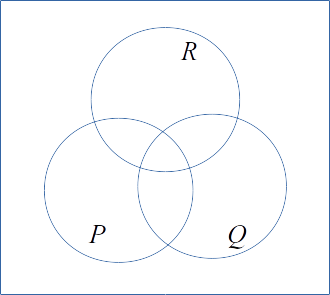
\includegraphics[width=2in]{midterm/circles.png}
\end{center}

\begin{enumerate}[(A)]
\item Copy the Venn diagram's circles in your solution and shade those regions in the diagram that make $E_0$ true
(the inside of each circle $P,Q,R$ shows that the respective variable $p,q,r$ is true and vice versa). 
\item In the truth table of $E_0$ how many entries are $\mathtt{True}$? 
\item Pick a Boolean expression that is equivalent to $E_0$ (if there are multiple, you can pick any one). 
Show by any method (equivalent transformations, case analysis, truth tables, etc.) that
the expression is equivalent to $E_0$. 
\end{enumerate}


Assume the following precedence order and associativity of the $5$ Boolean operations: 

\begin{tabular}{|l|l|l|} \hline
{\tt \textasciitilde{}a} & 1st precedence & right-associative \\ \hline
{\tt a/\textbackslash{}b} & 2nd precedence & right-associative \\ \hline
{\tt a\textbackslash{}/b} & 3rd precedence & right-associative \\ \hline
{\tt a<->b} & 4th precedence & left-associative \\ \hline
{\tt a->b} & 5th precedence & right-associative \\ \hline
\end{tabular}


\vspace{10pt}
{\bf Question 2 (15 \textperthousand{}).}

% Make transitive closure of the given flow graph - mark the predicate.
% How many pairs are satisfied? 
% Find predicate formulas that are satisfied.

\begin{center}
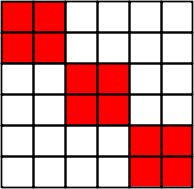
\includegraphics[width=1.0in]{midterm/relation.png}
\end{center}

\begin{enumerate}[(A)]
\item Does the predicate $P$ satisfy the logic formula:
$$\forall i \in A,\;P(i,i).$$
\item Does the predicate $P$ satisfy the logic formula:
$$\forall i \in A,\,\forall j \in A,\;P(i,j) \rightarrow P(j,i).$$
\item Does the predicate $P$ satisfy the logic formula:
$$\forall i,j,k \in A,\;P(i,j) \wedge P(j,k) \rightarrow P(i,k).$$
\item Does the predicate $P$ satisfy the logic formula:
$$\forall i,j \in A,\;P(i,j) \vee P(j,i).$$
\item Does the predicate $P$ satisfy the logic formula:
$$\forall i \in A,\, \exists j \in A,\;P(i,j).$$
\end{enumerate}

\vspace{10pt}
{\bf Question 3 (15 \textperthousand{}).}

Define the sequence 
$$S(n) = \sum\limits_{m=1}^n m^2.$$
We have $S(1) = 1^2 = 1$, $S(2) = 1^2 + 2^2 = 5$, and so on. 

\begin{enumerate}
\item Find the smallest $k$ such that $S(n)$ is in $O(n^k)$. 
\item Prove that $S(n)$ is in $O(n^k)$ by checking the 
definition or by finding a limit $S(n)/n^k$ when $n \rightarrow \infty$. 
\end{enumerate}


\vspace{10pt}
{\bf Question 4 (15 \textperthousand{}).}

Consider the following system of three congruences:
$$\left\{ \begin{array}{l}
x \equiv 1\;(\text{mod}\,5)\\
x \equiv 2\;(\text{mod}\,7)\\
x \equiv 3\;(\text{mod}\,9) 
\end{array} \right.$$

\begin{enumerate}
\item Does it have a solution? Will it have solution, even if we replace $1,2,3$ with other numbers
on the right sides of the equation.
\item Find an arithmetic progression ($a_1, d_1$) that solves the first two congruences?
\item Find an arithmetic progression ($a_2, d_2$) that solves the first three congruences?
\end{enumerate}


\vspace{10pt}
{\bf Question 5 (15 \textperthousand{}).}

Somebody has written an infinite periodic binary fraction on the board: 
$$\alpha = 0.(011110)_2 = 0.011110011110011110\ldots$$

\begin{enumerate}
\item Express the number $\beta = 0.01111001$ (the initial digits from $\alpha$) 
as a sum of some negative powers of $2$, i.e. show how to add up some of the numbers
$$\{ 2^{-1}, 2^{-2}, 2^{-3}, \ldots \}$$
in order to get $\beta$. 
\item Write the binary notation of $64\alpha$ (i.e. multiply the infinite $\alpha$ by 
$2^6$, where $6$ is the number of digits in the period). 
\item Write the binary notation for their difference: $64\alpha - \alpha = 63\alpha$. 
\item Express the value of $\alpha$ in decimal notation.
\end{enumerate}



\vspace{10pt}
{\bf Question 6 (25 \textperthousand{}).}
Among the people $A,B,C$ one is a truth-teller, 
the other two are liars. 
Every person ($A$, $B$, and $C$) has a closed box
in front of himself/herself. Exactly one of the 
boxes has a candy inside. $A,B,C$ know everything 
about each other and the location of candy.

Someone else (person $D$) approaches all of them. $D$ knows, who is 
person $A$,$B$,$C$ (it is written on their name-cards), but $D$ does
not know anything about their lying behavior or the location of the candy.
$D$ is allowed to ask YES/NO questions to one or more people.

\begin{enumerate}[(A)]
\item Can $D$ find out who has the candy by asking three questions?
\item Can $D$ find out who has the candy by asking two questions?
\item Can $D$ find out who has the candy by asking one question?
\end{enumerate}

Justify your answers (by construction or by showing that it is impossible).


\vspace{10pt}
{\bf Question 7 (25 \textperthousand{}).}

Assume that there is a Boolean expression $E$ with $n$ variables: 
$$E = E(a_1,a_2,\ldots,a_n).$$
The expression $E$ contains $2n$ Boolean operators (such as $\neg$, $\wedge$, $\vee$).
Variables $a_1,a_2,\ldots,a_n$ can independently take values 
$\mathtt{True}$ or $\mathtt{False}$.

Consider the following algorithm to find, if $E$ is a tautology by 
building the truth table \textendash{} either until we find a false value, or 
we establish that all values there are true.

{\bf (1)} \hspace{0.0in} For each assignment of $n$ truth values to $a_1,\ldots,a_n$:\\
{\bf (2)} \hspace{0.5in} For each of the $2n$ Boolean operators in $E$:\\
{\bf (3)} \hspace{1.0in} Compute the value of that Boolean operator (follow the precedence rules)\\
{\bf (4)} \hspace{0.5in} If $E$ has value $\mathtt{False}$:\\
{\bf (5)} \hspace{1.0in} Return ``$E$ is not a tautology.''\\
{\bf (6)} \hspace{0.5in} If $E$ has value $\mathtt{True}$:\\
{\bf (7)} \hspace{1.0in} Continue with another assignment of truth values on Line 1.\\
{\bf (8)} \hspace{0.0in} Return ``$E$ is a tautology.''

Find the worst-case runtime for this algorithm as an expression of $n$. 
Assume that evaluating any Boolean operator (

\vspace{10pt}
{\bf Question 8 (25 \textperthousand{}).}

We denote two real numbers by $p$ and $q$. 
Prove or disprove statements about the rational and irrational numbers. 

\begin{enumerate}[(A)]
\item If $p + q$ is rational, then either both $p,q$ are rational, or both are irrational. 
\item If $pq$ is rational, then either both $p,q$ are rational, or both are irrational. 
\item If $p^2$ and $q^2$ are both rational, then the product $(p+q)(p-q)$ is rational. 
\item If $p^3$ and $p^5$ are both rational, then $p$ is rational.
\item If $pq$ and $p+q$ are both rational, then $p$ and $q$ are also rational.
\end{enumerate}


\end{document}

